\newpage
\begin{appendices}
\section{Evaluation of Existing Machine-learning based Name Generation Approaches for Generating Test Names}
\label[appendix]{sec:pilot-study}

Recent machine-learning based approaches (e.g.,~\cite{alon2018code2seq, alon2019code2vec}) performe significantly better on method and class name generation than previous approaches (e.g.,~\cite{allamanis2015suggesting, zhang2016towards}).
%
However, it is unknown how well these machine-learning based approaches work in the context of generating names for unit tests.
%
To evaluate their performance for this task, we conducted a pilot study.

\subsection{Considered Name Generations Approaches}

%TODO[fixed] What are the ML techniques?  Why these ones?  How are they different?
As the state-of-the-art work on the topic of abstracting code to use it for name generation, \citeauthor{alon2018code2seq} proposed a series of novel approaches on representing code snippets as compositional paths or continuous distributed vectors~\cite{alon2018code2seq, alon2019code2vec}.
% TODO: You need to be careful here.  Is there really an evaluation comparing all of these appraoches  Pretty sure no one compared them against Zhang?  If not you can't say that it outperforms.  Instead you can say something like ``it appears''  Or you can limit the claim to what is actually compared against which I think is other approaches for general name generation.
After an initial review of the results of their approaches, their generated test names basically outperformed every existing name generation technique as far as we know~\cite{arcuri2014automated, ghafari2015automatically,pollock2010natural, pradel2018deepbugs, zhang2016towards, host2009debugging, schafer2008sound,allamanis2015suggesting, daka2017generating}.
%
The difference between the two approaches is that \texttt{Code2seq} encodes a code snippet to a set of compositional paths, and \texttt{Code2vec} encodes a code snippet to a fixed-length continuous vector.
%
Nonetheless, both of their approaches can make accurate prediction of Java method names.

\subsection{Considered Unit Tests}

\begin{table}[t]
\centering
\caption{Experimental Subjects.}
\begin{tabular}
{
  l
  l
  S[table-format=5.1]
  S[table-format=5.1]
}
\toprule
\multicolumn{1}{c}{\textbf{Project}} &
\multicolumn{1}{c}{\textbf{Version}} & 
\multicolumn{1}{c}{\textbf{LoC}} &
\multicolumn{1}{c}{\textbf{\# Tests}}
\\
\midrule
 Guice             & 9b371d3 &  183049  & 1280   \\
 Moshi             & dbed99d  &  22168  & 716   \\
 Picasso           & a087d26  &  11006  & 229  \\
 Fastjson          & e05f1f9  &  195511  & 4950   \\
 Guava             & 368c337  &  400801  & 13962  \\
 Mockito           & 22c82dc   &  59839 & 2145   \\
 Socket.io-client  & 661f1e7  &  9478  & 85  \\
 Scribejava        & ea42bc9  &  15184  & 110   \\
 ExoPlayer         & 79da521  &  172148  & 1510   \\
 Javapoet          & e9460b8  &  10755  & 302   \\
 Barbecue          & 44a8632  &  10760  & 170   \\
\bottomrule
\end{tabular}
\label{tab:subjectsForPilot}
\end{table}


To gather the tests we examined in our study, we started with the \num{11} Java projects \footnote{Same projects in the empirical study} shown in~\cref{tab:subjectsForPilot}.
%
In the table, the first column, \emph{Name}, shows the name of the project; the second column, \emph{Version}, shows the version of the project (either as a Git hash or version number); the fourth column, \emph{LoC}, shows the number of non-comment, non-blank lines of code as computed by SLOC count~\cite{nguyen2007sloc}; and the final column, \emph{\# Tests}, shows the number of unit tests in the project. In total, these \num{11} projects contain \num{25459} unit tests.
%
The first ten projects were randomly selected from the top \num{50} Java projects hosted on Github~\cite{top50projects}.
%
Because these projects encompass a variety of domains (e.g., JavaPoet is a library for generating Java programmatically and ExoPlayer is a media player for Android) and have many contributors (e.g., Moshi’s test suite contains contributions from \num{8} different people), their tests are more likely to be representative of tests in general which helps mitigate a potential threat to validity.
%
In addition, we also included Barbecue, a commonly used subject in the testing literature (e.g.,~\cite{zhang2015automatically, zhang2016towards, wu2020pattern}).
% TODO: you could provide more details here.
\num{15400} tests were randomly selected from different test classes under different projects to evaluate both \texttt{Code2seq} and \texttt{Code2vec}.


\subsection{Data and Discussion}

To generate the data necessary for investigating the quality of the generated names, we ran \texttt{Code2seq} and \texttt{Code2vec} on the set of \num{15400} tests.
%
Both \texttt{Code2seq} and \texttt{Code2vec} were run on a MacBook Pro (2.4GHz Intel i5 processor and 8GB RAM) with MacOS Mojave \footnote{Same machine in the empirical study}, Tensorflow 1.13.1 and Tensorflow 2.0.0, respectively.
% Were you doing this locally or did you use the web interface?  This just seems really long.  Really just the execution time is what matters.
It took roughly \num{25} hours to both configure necessary environment and generating names for tests.

%TODO: I want to see the bodies of these tests.  You want people to be able to see how the similarities in the bodies.
\begin{figure}[t]
\centering
\begin{subfigure}[b]{1.0\textwidth}
\centering
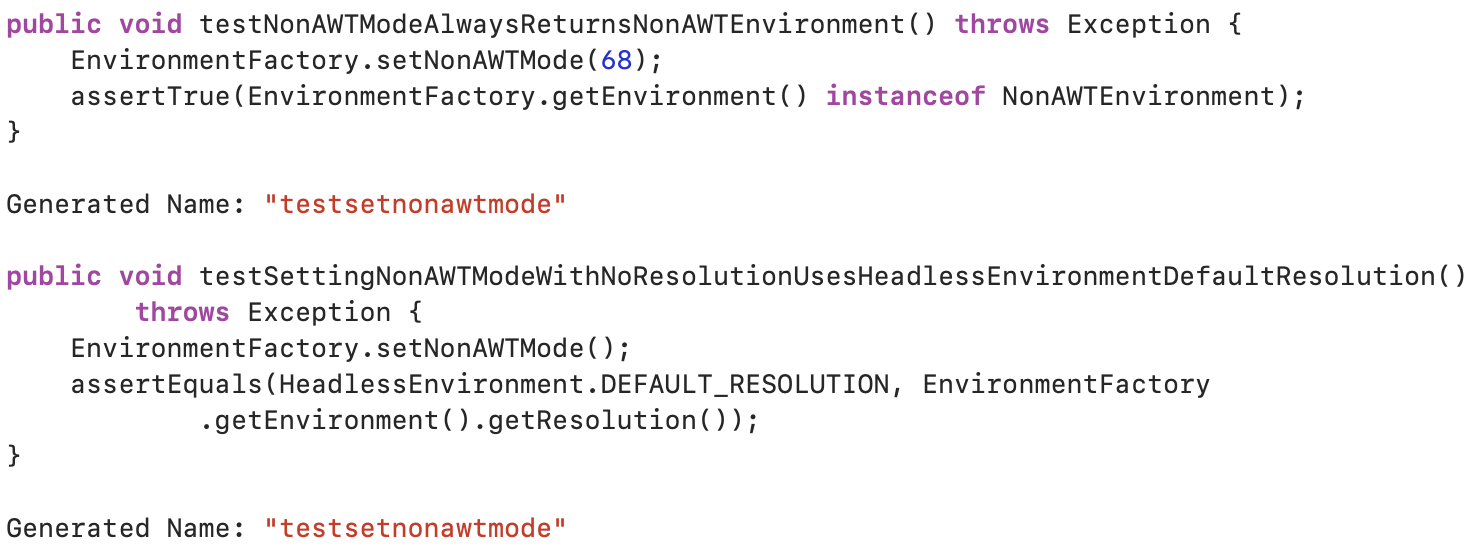
\includegraphics[scale=0.5]{figures/dup1.png}
\caption{Generated names by \texttt{Code2seq}.}
\label{fig:generated1}
\end{subfigure}\\
\vspace{0.2cm}
\begin{subfigure}[b]{0.5\textwidth}
\centering
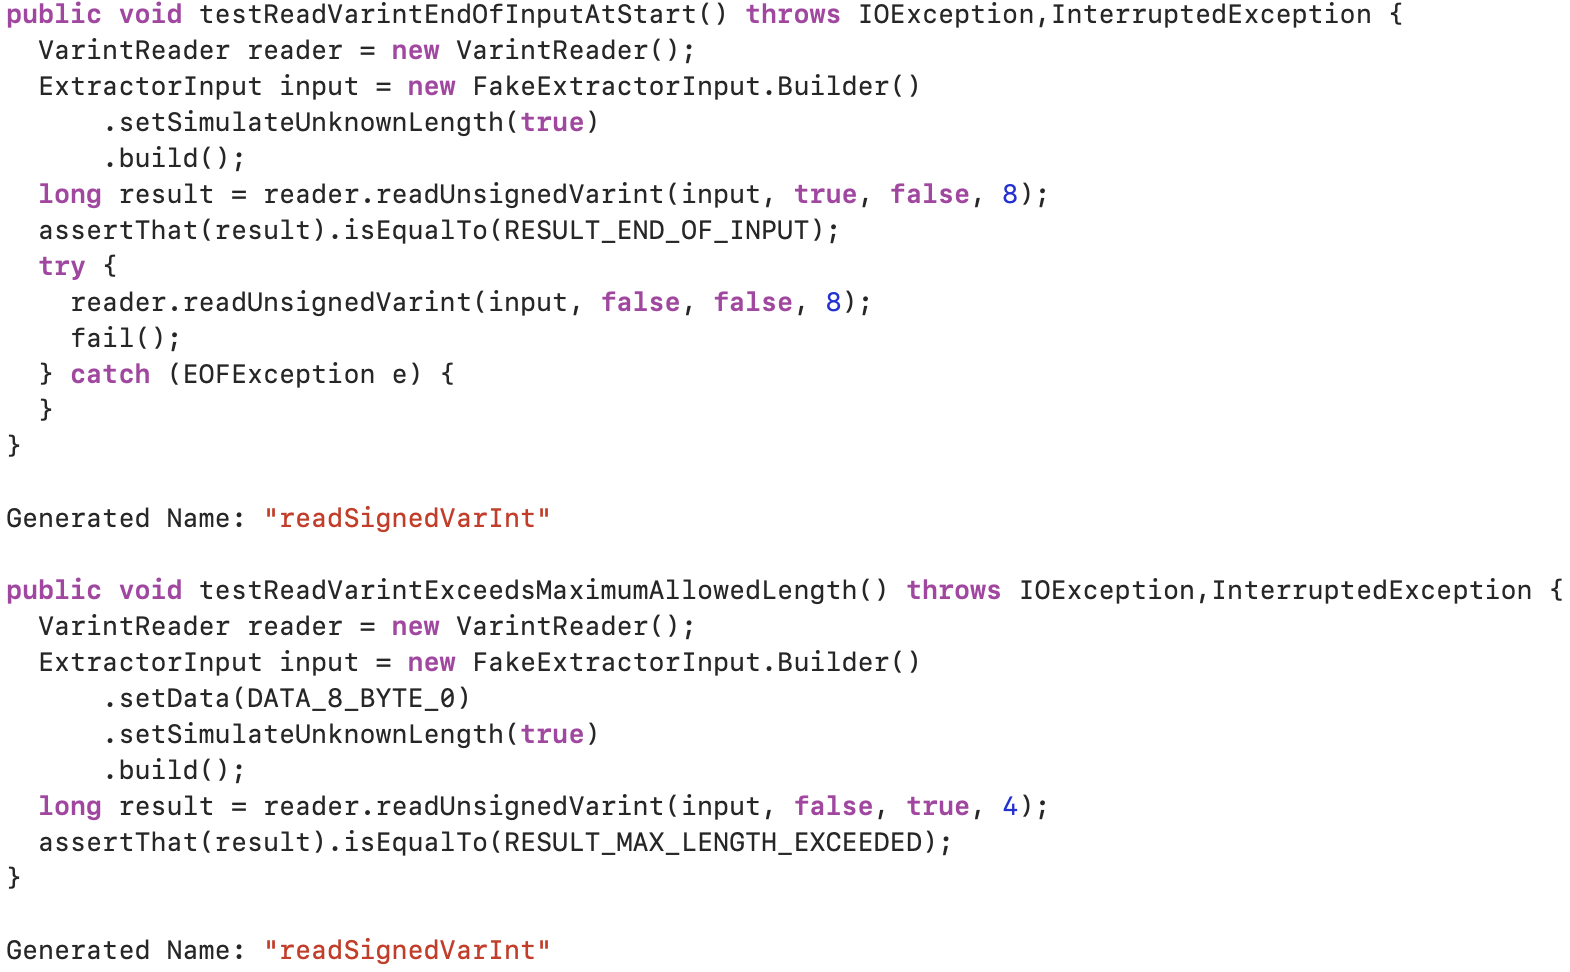
\includegraphics[scale=0.5]{figures/dup2.png}
\caption{Generated names by \texttt{Code2vec}.}
\label{fig:generated2}
\end{subfigure}
\caption{Example of generated names.}
\label{fig:duplicate-names}
\end{figure}


In~\cref{fig:generated1}, it shows two test names generated for test from Scribejava using \texttt{Code2seq}.
%
For example, \texttt{extract\-With\-Empty\-Response} is generated for \texttt{should\-Throw\-Exception\-If\-Response\-Is\-Empty\-String}.
%
In~\cref{fig:generated2}, it shows two test names generated for ExoPlayer by using \texttt{Code2vec}.
%
For another example, \texttt{accumulate} is generated for \texttt{test\-Merge}.


Initially, our manual examination of the names was posiitve.
%
The names appeared to be descriptive and were similiar in format to existing test names.
%
However, we soon realized that both approaches frequently generated duplicate names for different tests in the same class.



For example, \texttt{extract\-with\-empty\-response} is repeated \num{3} times, and \texttt{accumulate} is repeated \num{4} times.

% TODO: I would like to see a table here.
% FOr each project show how many times a name is repeated in a test class.

% Then Update the discussion to match.



We collected and analyzed the generated test names from both \texttt{Code2seq} and \texttt{Code2vec}.
%
If there are many generated test names that are repeated at least once in its associated test class, it is necessary to develop a uniqueness-focused approach to solve the problem of duplication.
%
The collected data is shown in a shared document~\cite{CodeResult}.
%
It shows hundreds or thousands of duplicate names were generated for each project during their name generation process. 
%
For example, \texttt{Code2seq} produced \num{240} duplicate test names for ExoPlayer, and \num{57} out of \num{187} test classes in ExoPlayer contain more than one duplicate names.
%
For another example, \texttt{Code2vec} produced \num{1161} duplicate test names for Guava, and \num{209} out of \num{458} test classes in Guava contain more than one duplicate names.
%
Both state-of-the-art approaches produced a significant number of duplicate names when performing their automated name generation on unit tests.
%
This result indicates there is a need to develop a uniqueness-focused approach that can extract unique attributes of tests to generate descriptive names.


\end{appendices}